%!TEX root = notes.tex


\chapter{Background}

Our starting point is, for any positive integer $d \in \field{N}$, the Cartesian products:
\begin{equation*}
\field{R}^d = \field{R} \times \overset{(d)}{\dotsm} \times \field{R} =\{ (x_1, \dotsc, x_d) : x_k \in \field{R} \text{ for } 1\leq k \leq d\}.
\end{equation*}
These sets, endowed with the operations of addition and scalar multiplication, have the structure of a \emph{vector field}:
\begin{description}
	\item[Addition] For $\x = (x_1, \dotsc, x_d), \y = (y_1, \dotsc, y_d) \in \field{R}^d$, 
	\begin{equation*}
	\x + \y = (x_1+y_1, \dotsc, x_d+y_d) \in \field{R}^d.
	\end{equation*}
	\item[Scalar multiplication] For $\x \in \field{R}^d$ and $\lambda \in \field{R}$, 
	\begin{equation*}
	\lambda \cdot \x = \lambda \x = (\lambda x_1, \dotsc, \lambda x_d) \in \field{R}^d.
	\end{equation*}
\end{description}
Given $\x, \y, \z \in \field{R}^d$, $\lambda, \mu \in \field{R}$,
\begin{enumerate}
	\item The addition is commutative: $\x + \y = \y + \x$.
	\item Existence of identity elements for addition: Let $\boldsymbol{0} = (0, \dotsc, 0)$. $\x + \boldsymbol{0} = \x$. 
	\item The addition is associative: $\x + (\y + \z) = (\x + \y) + \z$.
	\item Existence of inverse elements for addition: If $\x = (x_1, \dotsc, x_d)$, the element $-\x = (-x_1, \dotsc, -x_d)$ satisfies $\x + (-\x) = \boldsymbol{0}$.  We write $\x - \y$ instead of $\x + (-\y)$.
	\item Scalar multiplication is compatible with field multiplication: $\lambda (\mu \x) = (\lambda \mu) \x$.
	\item Existence of identity for scalar multiplication: $1 \cdot \x = \x$.
	\item Scalar multiplication is distributive with respect to addition: $\lambda (\x + \y) = \lambda \x + \lambda \y$.
	\item Scalar multiplication is distributive with respect to field addition: $(\lambda + \mu)\x = \lambda \x + \mu\x$.
\end{enumerate}
A \emph{basis} of $\field{R}^d$ is any finite set $\{ \boldsymbol{b}_k : 1\leq k \leq d \}$ satisfying two properties:
\begin{description}
\item [Spanning property] For all $\x \in \field{R}^d$ there exist $d$ scalars $\{ \lambda_1, \dotsc, \lambda_d \}$ so that $\x = \sum_{k=1}^d \lambda_k \boldsymbol{b}_k$.
\item [Linear independence] If $\{ \lambda_1, \dotsc, \lambda_d\}$ satisfy $\sum_{k=1}^d \lambda_k \boldsymbol{b}_k = \boldsymbol{0}$, then it must be $\lambda_k=0$ for all $1\leq k \leq d$.
\end{description}

\begin{problem}\label{problem:basisRd}
Define in $\field{R}^d$, for each $1\leq k \leq d$, the element $\e_k$ to be the ordered $d$-tuple with $k$-th entry equal to one, and zeros on all other entries.
\begin{enumerate}
	\item Prove that $\{ \e_k : 1\leq k \leq d\}$ is a basis for $\field{R}^d$.
	\item Set $\boldsymbol{b}_k = \e_k - \e_{k+1}$ for $1\leq k < d$, $\boldsymbol{b}_d = \e_d$.  Is $\{ \boldsymbol{b}_k : 1\leq k \leq d\}$ a basis for $\field{R}^d$?
\end{enumerate}
\end{problem}

\section{Functions}

Given sets $X, Y$, we define a \emph{function} $f\colon X \to Y$ to be a subset of $X \times Y$ subject to the following condition: for every $\x \in X$ there is exactly one element $\y \in Y$ such that the ordered pair $(\x, \y)$ is contained in the subset defining $f$. The sets $X$ and $Y$ are called respectively the \emph{domain} and \emph{codomain} of $f$.  

If $A$ is any subset of the domain $X$, then $f(A)$ is the subset of the codomain $Y$ consisting of all images of elements of $A$. We say that $f(A)$ is the \emph{image} of $A$ under $f$. The image of $f$ is given by $f(X)$.  

If $Y \subset \field{R}$, we say that the function $f$ is real-valued.  For a real-valued function $f\colon \field{R}^d \to \field{R}$, we may regard the corresponding ordered pairs $(\x, y) \in \field{R}^d\times\field{R}$ as points in a $(d+1)$--dimensional space.  We call this set the \emph{graph} of $f$.

The \emph{inverse image} of a subset $B$ of the codomain $Y$ under a function $f$ is the subset of the domain $X$ defined by $f^{-1}(B) = \{ \x \in X : f(x) \in B\}$.

For sets $X, Y, Z$, the \emph{function composition} of $f\colon X \to Y$ with $g\colon Y \to Z$ is the function $g\circ f\colon X \to Z$ defined by $\big( g \circ f \big)(\x) = g \big( f(\x) \big)$.

Unless specifically stated otherwise, all functions in these notes are real-valued functions $f \colon \field{R}^d \to \field{R}$.

\begin{example}[Linear Functions]\label{example:linearFunction}
We say that a real-valued function is \emph{linear} if it preserves the operations in $\field{R}^d$: 
\begin{equation*}
f(\x + \lambda \y) = f(\x) + \lambda f(\y) \text{ for }\x, \y \in \field{R}^d, \lambda \in \field{R}.
\end{equation*}

With this definition, the function $f(x) = 3x$ is indeed a linear function, but $g(x)=3x+5$ is not!  
It is not hard to see that the only linear constant function is $f(x) = 0$ (since $f(0)=f(x-x)=f(x)-f(x)=0$).  For a non-constant linear function $f(x)$, it is also easy to see that the image is the whole real line.
\end{example}

\begin{example}[Convex Functions]\label{example:convexFunction}
A subset $C \subset \field{R}^d$ is said to be \emph{convex} if for every $\x, \y \in C$, and every $\lambda \in [0,1]$, the point $\lambda \x + (1-\lambda) \y$ is also in $C$.   Given such a convex set, we say that a real-valued function $f \colon C \to \field{R}$ is \emph{convex} if 
\begin{equation*}
f\big(\lambda \x + (1-\lambda)\y\big) \leq \lambda f(\x) + (1-\lambda) f(\y)
\end{equation*}
\begin{figure}[ht!]\label{figure:convexFunction}
% \begin{center}
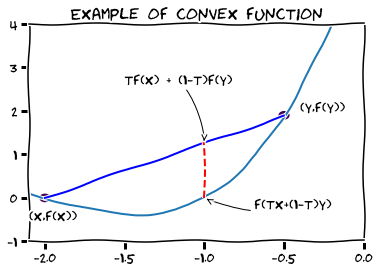
\includegraphics[width=0.5\linewidth]{convexFunction.png}
% \end{center}
% \caption{In convex functions, the segment joining two points of the graph is always above the graph.}
\end{figure}
If instead we have $f\big(\lambda \x + (1-\lambda)f(\y)\big) < \lambda f(\x) + (1-\lambda) f(\y)$ for $0<\lambda<1$, we say that the function is \emph{strictly convex}.  A function $f$ is said to be \emph{concave} (resp.~\emph{strictly concave}) if $-f$ is convex (resp.~strictly convex).
\end{example}

\begin{example}[Rosenbrock Functions]\label{example:Rosenbrock2}
Given strictly positive parameters $a,b > 0$, consider the $(a,b)$--Rosenbrock function $\mathcal{R}_{a,b}\colon \field{R}^2 \to \field{R}$ defined by:
\begin{equation*} 
\mathcal{R}_{a,b}(x_1, x_2) = (a-x_1)^2 + b(x_2-x_1^2)^2.
\end{equation*}
The image of $\mathcal{R}_{a,b}$ is the interval $[0,\infty)$.  Indeed, note first that $\mathcal{R}_{a,b}(\x) \geq 0$ for all $\x \in \field{R}^2$.  Zero is attained: $\mathcal{R}_{a,b} (a,a^2) = 0$.  Note also that $\mathcal{R}_{a,b}(x_1,0) = (a-x_1)^2 + bx_1^4$ is a polynomial of degree 4, hence unbounded for $x_1 \in \field{R}$.
Figure \ref{figure:Rosenbrock} illustrates a contour plot with several level lines of $\mathcal{R}_{1,1}$ on the domain $D = [-2,2] \times [-1,3]$, as well as its graph
\begin{figure}[ht!]\label{figure:Rosenbrock}
\begin{tabular}{cc}
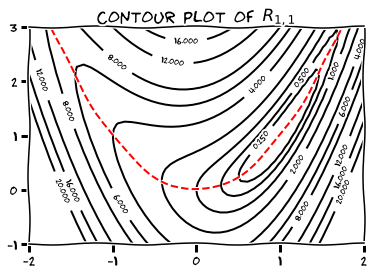
\includegraphics[width=0.5\linewidth]{rosenbrockContour} &
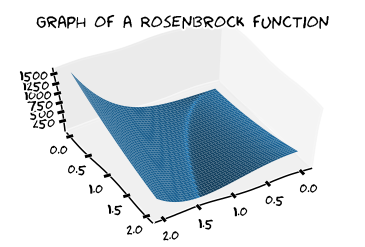
\includegraphics[width=0.5\linewidth]{rosenbrockGraph}
\end{tabular}
% \caption{Details of the graph of $\mathcal{R}_{1,1}$}
\end{figure}
\end{example}



This is a good spot to introduce the goal of these notes.  The main purpose of \emph{optimization} is the search for \emph{extrema} of real-valued functions.  Given a set $D \subset \mathbb{R}^d$, and a real-valued function $f\colon D \to \field{R}$, we say that a point $\xstar \in D$ is:
\begin{enumerate}
	\item A \emph{global minimum} for $f$ on $D$ if $f(\xstar) \leq f(\x)$ for all $\x \in D$.
	\item A \emph{global maximum} for $f$ on $D$ if $f(\xstar) \geq f(\x)$ for all $\x \in D$.
	\item A \emph{strict global minimum} for $f$ on $D$ if $f(\xstar) < f(\x)$ for all $\x \in D \setminus \{ \xstar \}$.
	\item A \emph{strict global maximum} for $f$ on $D$ if $f(\xstar) > f(\x)$ for all $\x \in D \setminus \{ \xstar \}$.
	\item A \emph{local minimum} for $f$ on $D$ if there exists $\delta>0$ so that  $f(\xstar) \leq f(\x)$ for all $\x \in B_\delta(\xstar)\cap D$.
	\item A \emph{local maximum} for $f$ on $D$ if there exists $\delta>0$ so that  $f(\xstar) \geq f(\x)$ for all $\x \in B_\delta(\xstar)\cap D$.
	\item A \emph{local minimum} for $f$ on $D$ if there exists $\delta>0$ so that  $f(\xstar) < f(\x)$ for all $\x \in B_\delta(\xstar)\cap D$, $\x \neq \xstar$.
	\item A \emph{local maximum} for $f$ on $D$ if there exists $\delta>0$ so that  $f(\xstar) > f(\x)$ for all $\x \in B_\delta(\xstar)\cap D$, $\x \neq \xstar$.
\end{enumerate}

Let's play around with some more examples of functions, before we proceed to techniques for finding extrema:

\begin{example}[Bilinear Forms]\label{example:BilinearForm}
Let $\boldsymbol{A} = \big[ a_{jk} \big]_{j,k=1}^d$ be a square matrix with real coefficients.  Considering elements in $\field{R}^d$ as horizontal matrices, and by means of matrix products, we construct functions $\bilinear{A} \colon \field{R}^d \times \field{R}^d \to \field{R}$ given by
\begin{equation*}
\bilinear{A}(\x, \y) = \begin{bmatrix} x_1 \dotsb x_d \end{bmatrix} \begin{bmatrix} a_{11} &\dotsb &a_{1d} \\ \vdots & \ddots & \vdots \\ a_{d1} &\dotsb &a_{dd} \end{bmatrix} \begin{bmatrix} y_1 \\ \vdots \\ y_d \end{bmatrix}
\end{equation*}
We call functions constructed in this way \emph{bilinear forms}.
\end{example}

\begin{problem}\label{problem:BilinearForm}
Prove that, if the associated matrix is symmetric ($\boldsymbol{A} = \transpose{\boldsymbol{A}}$), then $\bilinear{A}(\x,\y) = \bilinear{A}(\y,\x)$ for all $\x, \y \in \field{R}^d$.
\end{problem}

\begin{example}[Quadratic Forms]\label{example:QuadraticForm}
Each symmetric bilinear form has an associated \emph{quadratic form}: A function $\quadratic{A} \colon \field{R}^d \to \field{R}$ constructed as follows:
\begin{equation*}
\quadratic{A}(\x) = \bilinear{A}(\x,\x) = \begin{bmatrix} x_1 \dotsb x_d \end{bmatrix} \begin{bmatrix} a_{11} &\dotsb &a_{1d} \\ \vdots & \ddots & \vdots \\ a_{1d} &\dotsb &a_{dd} \end{bmatrix} \begin{bmatrix} x_1 \\ \vdots \\ x_d \end{bmatrix}
\end{equation*}
We say that the quadratic form (or the associated matrix) is:
\begin{description}
\item[positive definite] if $\quadratic{A}(\x) > 0$ for all $\x \in \field{R}^d \setminus \{ \boldsymbol{0} \}$.
\item[positive semidefinite] if $\quadratic{A}(\x)\geq 0$ for all $\x \in \field{R}^d$.
\item[negative definite] if $\quadratic{A}(\x) < 0$ for all $\x \in \field{R}^d \setminus \{ \boldsymbol{0} \}$.
\item[negative semidefinite] if $\quadratic{A}(\x) \leq 0$ for all $\x \in \field{R}^d$.
\item[indefinite] if there exist $\x, \y \in \field{R}^d$ so that $\quadratic{A}(\x) \quadratic{A}(\y) < 0$. 
\end{description}
\end{example}

\begin{example}[Inner products]\label{example:innerprod}
We say that a symmetric bilinear form $\bilinear{A}$ is an \emph{inner product} if its associated quadratic form is positive definite.  By extension, we call an inner product any function $\mathcal{F} \colon \field{R}^d \times \field{R}^d \to \field{R}$ that satisfies the following four properties for all $\x, \y, \z \in \field{R}^d, \lambda \in \field{R}$:
\begin{enumerate}
\item $\mathcal{F}(\x+\y, \z) = \mathcal{F}(\x, \z) + \mathcal{F}(\y, \z)$.
\item $\mathcal{F}(\lambda \x, \y) = \lambda \mathcal{F}(\x, \y)$.
\item $\mathcal{F}(\x, \y) = \mathcal{F}(\y, \x)$.
\item $\mathcal{F}(\x, \x) \geq 0$, $\mathcal{F}(\x, \x) = 0$ if and only if $\x = \boldsymbol{0}$.
\end{enumerate}
\end{example}

\begin{problem}\label{problem:innerprodRd}
Prove that $\langle \cdot, \cdot \rangle \colon \field{R}^d \times \field{R}^d \to \field{R}$ given by
\begin{equation*}
\langle \x, \y \rangle = \sum_{k=1}^d x_k y_k
\end{equation*}
is an inner product.  What is the matrix associated to its corresponding bilinear form?
\end{problem}

\begin{problem}\label{problem:linearFunction}
Prove that, if $f$ is a linear function, then there exist a unique $\boldsymbol{a}_0 \in \field{R}^d$ so that $f(\x)=\langle \boldsymbol{a}_0, \x \rangle$ for all $\x \in \field{R}^d$.
\end{problem}

\begin{problem}\label{problem:affineFunction}
We say that $\tau\colon \field{R}^d \to \field{R}^d$ is a translation if there exist a fixed $\x_0 \in \field{R}^d$ so that $\tau(\x) = \x + \x_0$ for all $\x \in \field{R}^d$.

An \emph{affine function} $h\colon \field{R}^d \to \field{R}$ is a composition of a linear function $f\colon \field{R}^d \to \field{R}$ with a translation $\tau\colon \field{R} \to \field{R}$.

Prove that for each affine function $h$ there exist a unique $\boldsymbol{a}_0 \in \field{R}^d$ and a unique $\lambda_0 \in \field{R}$ so that $h(\x) = \lambda_0 + \langle \boldsymbol{a}_0, \x \rangle$ for all $\x \in \field{R}^d$.  Use this result to prove that the graph of an affine function is a hyperplane in $\field{R}^{d+1}$.
\end{problem}

\begin{example}[Norms]\label{example:norm}
A \emph{norm} in $\field{R}^d$ is a function $\norm{\cdot} \colon \field{R}^d \to \field{R}$ that satisfies the following properties:
For all $\x, \y \in \field{R}^d$, and for all $\lambda \in \field{R}$,
\begin{enumerate}
	\item $\norm{\x} \geq 0$.
	\item $\norm{\x} = 0$ if and only if $\x = \boldsymbol{0}$
	\item $\norm{ \lambda \x} = \abs{\lambda} \norm{\x}$.
	\item Triangle inequality: $\norm{\x + \y} \leq \norm{\x} + \norm{\y}$.
\end{enumerate}
\end{example}

\begin{problem}\label{problem:norm}
Consider the function $\norm{\cdot} \colon \field{R}^d \to \field{R}$ defined by 
\begin{equation*}
\norm{\x} = \langle \x, \x \rangle^{1/2}.
\end{equation*}
\begin{enumerate}
	\item Prove that $\norm{\cdot}$ is a norm
	\item Prove the \emph{Cauchy-Schwartz inequality}: For all $\x, \y \in \field{R}^d$, 
	\begin{equation*}
	\big\lvert \langle \x, \y \rangle \big\rvert \leq \norm{\x} \norm{\y}.
	\end{equation*}
\end{enumerate}
\end{problem}


\section{Topology}
The norm introduced in Example \ref{example:norm} induces a \emph{metric} $\dist \colon \field{R}^d \times \field{R}^d \to \field{R}^d$ on the space $\field{R}^d$: 
\begin{equation*}
\dist(\x,\y) = \norm{\x - \y} \text{ for any }\x, \y \in \field{R}^d.
\end{equation*}
Metrics allow us to measure distance between elements.  These are the four main properties of these objects:  Given $\x, \y, \z \in \field{R}^d$,
\begin{description}
	\item[Separation property] $\dist(\x,\y) \geq 0$.
	\item[Identity of indiscernibles] $\dist(\x, \y) = 0$ if and only if $\x = \y$.
	\item[Symmetry] $\dist(\x, \y) = \dist(\y, \x)$.
	\item[Triangle inequality] $\dist(\x,\z) \leq \dist(\x,\y) + \dist(\y,\z)$. 
\end{description}
Metric spaces like $\big( \field{R}^d, \dist(\cdot,\cdot) \big)$ inherit a \emph{topology} in a natural manner, as explained below.

We define the \emph{open ball} of radius $r>0$ about $\x$ as the set $B_d(\x,r) = \big\{ \y \in \field{R}^d : \norm{\x- \y} < r \big\}$.  We say $\x$ is an interior point of $D \subset \field{R}^d$ if $\x \in D$ and there exists $r>0$ so that $B_d(\x, r) \subset D$.  A subset $G \subset \field{R}^d$ is said to be open if all its points are interior.

A \emph{neighborhood} of the point $\x$ is any subset of $\field{R}^d$ that contains an open ball about $\x$ as subset. 

A \emph{sequence} $\sequence{\x}{n}$ in $\field{R}^d$ is an enumerated collection of elements of $\field{R}^d$ in which repetitions are allowed.  A sequence is said to \emph{converge} to the limit $\x \in \field{R}^d$ if and only if for every $\varepsilon>0$ there exists $N=N(\varepsilon) \in \field{N}$ so that $\norm{\x_n - \x} < \varepsilon$ for all $n \geq N$.  We write then 
\begin{equation*}
\x = \lim_{n\to\infty} \x_n = \lim_n \x_n, \text{ or } \lim_{n\to\infty} \norm{\x_n - \x} = \lim_n \norm{\x_n - \x} = 0.
\end{equation*}

We say that $\sequence{\x}{n}$ is a \emph{Cauchy sequence} if for every $\varepsilon>0$ there exists $N = N(\varepsilon) \in \field{N}$ so that for any $m,n \geq N$, $\norm{\x_n - \x_m} < \varepsilon$.  

\begin{problem}[Completeness of Euclidean spaces]\label{problem:Rdcomplete}
Prove that all Cauchy sequences converge in $\field{R}^d$ (\textbf{Hint}: this is direct consequence of the completeness of $\field{R}$, which you should also prove).
\end{problem}

The complement of an open set is called \emph{closed}. In $\field{R}^d$, all subsets $F$ are closed if and only if they are \emph{sequentially closed}: If $\x_n\in F$ for all $n \in \field{N}$ and $\lim_n \norm{\x_n - \x} = 0$, then $\x \in F$.

We say $D$ is \emph{bounded} if there exists $M>0$ so that $D \subset B_d(\boldsymbol{0}, M)$.  A bounded and closed subset of $\field{R}^d$ is called \emph{compact}.

\begin{theorem}[Bolzano-Weierstrass]\label{theorem:BolzanoWeierstrass}
Every sequence in a compact subset $K \subset \field{R}^d$ contains a convergent subsequence.
\end{theorem}

\begin{problem}\label{problem:BolzanoWeierstrass}
Prove Theorem \ref{theorem:BolzanoWeierstrass} for a closed interval $K=[a,b] \subset \field{R}$.
\end{problem}

\section{Analysis}

A real-valued function $f$ is said to be \emph{continuous} at $\x_0$ if for any $\varepsilon>0$ there exists $\delta = \delta(\varepsilon)>0$ so that $\abs{f(\x) - f(\x_0)} < \varepsilon$ for all $x \in B_d(\x_0, \delta)$.

Equivalently, $f$ is continuous at $\x_0$ if $\lim_n f(\x_n) = f(\x_0)$ for any sequence $\sequence{\x}{n}$ satisfying $\lim_n \x_n = \x_0$.  

We say that $f$ is continuous in $D \subset \field{R}^d$ if $f$ is continuous at all points $\x \in D$.

The image of a continuous functions enjoys nice properties, which are key to the pursue of extrema.  Let's start with two basic Theorems.

\begin{theorem}[Bounded Value Theorem]\label{theorem:BVT}
The image $f(K)$ of a continuous real-valued function $f \colon \field{R}^d \to \field{R}$ on a compact set $K$ is bounded: there exists $M>0$ so that $\abs{ f(\x) } \leq M$ for all $\x \in K$.
\end{theorem}

\begin{theorem}[Extreme Value Theorem]\label{theorem:EVT}
A continuous real-valued function $f \colon K \to \field{R}$ on a compact set $K \subset \field{R}^d$ takes on minimal and maximal values on $K$.
\end{theorem}

Theorem \ref{theorem:EVT} guarantees the existence of global \emph{extrema} (maxima/minima) for continuous real-valued functions over compact subsets.  What if we do not have compactness?

\begin{example}[Coercive Functions]
A continuous real-valued function $f\colon \field{R}^d \to \field{R}$ is said to be \emph{coercive} if the values of $f(\x)$ cannot remain bounded on any non-bounded set $A\subset \field{R}^d$: 
\begin{equation*}
\lim_{\norm{\x} \to \infty} = +\infty.
\end{equation*}
A coercive function always has a global minimum.  Indeed: since $f$ is coercive, there exists $r>0$ so that $f(\x) > f(\boldsymbol{0})$ for all $\x$ satisfying $\norm{\x}>r$.  On the other hand, the set $K_r = \{ \x \in \field{R}^d : \norm{x} \leq r \}$ is compact.  The continuity of $f$ guarantees a global minimum $\xstar \in K_r$ with $f(\xstar) \leq f(\boldsymbol{0})$.  It is then $f(\xstar) \leq f(\x)$ for all $\x \in \field{R}^d$ trivially.
\end{example}


How about local extrema?   Continuity may not be enough:

A real-valued function $f$ is said to be \emph{differentiable} at $\x_0$ if there exists a linear function $J\colon \field{R}^d \to \field{R}$ so that 
\begin{equation*}
\lim_{\boldsymbol{h} \to \boldsymbol{0}} \frac{\abs{f(\x_0+h)-f(\x_0)-J(\boldsymbol{h})}}{\norm{\boldsymbol{h}}} = 0
\end{equation*}

For any differentiable real-valued function $f$ at a point $\x$ of its domain, the corresponding linear function in the definition above guarantees a tangent hyperplane to the graph of $f$ at $\x$.  It is the behavior of the interaction of the rest of the graph with this hyperplane what will give us clues to the nature of possible extrema.

\begin{figure}[ht!]\label{figure:extrema}
\begin{tabular}{cc}
%  &
% 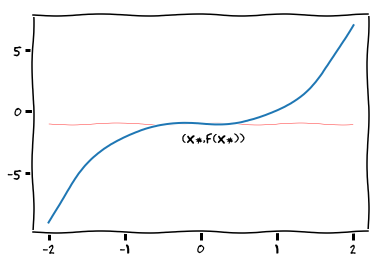
\includegraphics[width=0.45\linewidth]{x3.png}
\begin{tikzpicture}
\draw [white] (-2,-2) rectangle (2,2);
\draw (0,0) node{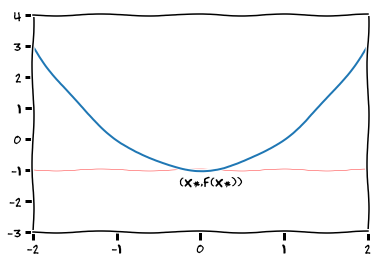
\includegraphics[width=0.5\linewidth]{x2.png}};
% \draw [smooth, samples=100, domain=-1.732:1.732, blue, ultra thick, variable=\t] plot({\t}, {\t*\t-1});
% \draw[thick] (-2,-1) -- (2,-1);
\draw[fill=blue] (0.1,-0.65) circle (2pt); 
% \draw (0.1,-1.25) node[scale=0.7] {$\big( \xstar, f(\xstar) \big)$};
\end{tikzpicture} &
\begin{tikzpicture}
\draw [white] (-2,-2) rectangle (2,2);
\draw (0,0) node{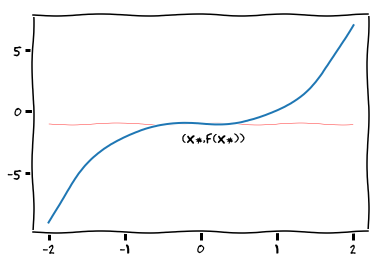
\includegraphics[width=0.5\linewidth]{x3.png}};
% \draw [smooth, samples=100, domain=-1:1.442, blue, ultra thick, variable=\t] plot({\t}, {\t*\t*\t-1});
% \draw[thick] (-2,-1) -- (2,-1);
\draw[fill=blue] (0.1,0.125) circle (2pt); 
% \draw (0.1,-0.2) node[scale=0.7] {$\big( \xstar, f(\xstar) \big)$};
\end{tikzpicture}
\end{tabular}
\caption{On the left: the function is locally \emph{above} the tangent hyperplane at $\big(\xstar, f(\xstar)\big)$.  We have a local minimum at that location.  On the right, the graph crosses the tangent hyperplane.  We have no extrema at that location.}
\end{figure}

\begin{example}\label{example:derivatives}
Consider a real-valued function $f\colon \field{R} \to \field{R}$ of a real variable. To prove differentiability at a point $x_0$, we need a linear function: $J(h)=ah$ for some $a\in \field{R}$. Notice how in that case, 
\begin{equation*}
\frac{\abs{f(x_0+h)-f(x_0)-J(h)}}{\abs{h}} = \left\lvert \frac{f(x_0)-f(x_0)}{h} - a \right\lvert;
\end{equation*}
therefore, we could pick $a = \lim_{h\to 0} h^{-1}\big( f(x_0+h) - f(x_0) \big)$---this is the definition of derivative we learned in Calculus.
\end{example}

\begin{problem}\label{problem:gradient}
Let $f\colon \field{R}^d \to \field{R}$ be a real-valued function.  To prove that $f$ is differentiable at a point $\x_0 \in \field{R}^d$ we need a linear function $J(h) = \langle \boldsymbol{a}, h \rangle$ for some $\boldsymbol{a} \in \field{R}^d$.  Prove that in this case, we can use
\begin{equation*}
\boldsymbol{a} = \gradient{f}(\x_0)= \bigg( \frac{\partial f}{\partial x_1}(\x_0), \dotsc, \frac{\partial f}{\partial x_d}(\x_0) \bigg).
\end{equation*}
\end{problem}

\begin{example}[Weierstrass Function]\label{example:WeierstrassFunction}
For any positive real numbers $a, b$ satisfying $0<a<1<b$ and $ab \geq 1$, consider the Weierstrass function $\mathcal{W}_{a,b} \colon \field{R} \to \field{R}$ given by 
\begin{equation*}
\mathcal{W}_{a,b}(x) = \sum_{n=0}^\infty a^n \cos(b^n \pi x)
\end{equation*}
This function is continuous everywhere, yet \emph{nowehere} differentiable!  For a proof, see e.g.~\cite{hardy1916weierstrass}
\begin{figure}[ht!]
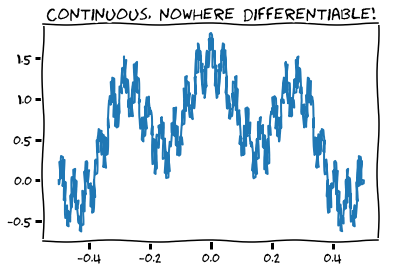
\includegraphics[width=0.5\linewidth]{weierstrass.png}
\caption{Detail of the graph of $\mathcal{W}_{0.5, 7}$}
\end{figure}
\end{example}

It is possible to extend the notion to higher derivatives.  We would say, for instance, that a function is \emph{twice differentiable} if the derivative is differentiable.  For the case of such a real-valued function $f \colon \field{R}^d \to \field{R}$, this would mean in particular that all second partial derivatives exist, and are continuous over the domain of $f$.

We define for these functions the \emph{Hessian} of $f$ at $\x \in D$ to be the following matrix of second partial derivatives:
\begin{equation*}
\Hess{f}(\x) = \begin{bmatrix}
\frac{\strut\partial^2 f}{\strut\partial x_1^2}(\x) & \frac{\strut\partial^2 f}{\strut\partial x_1 \partial x_2}(\x) &\dotsb &\frac{\strut\partial^2 f}{\strut\partial x_1 \partial x_d}(\x) \\
&&&\\
\frac{\strut\partial^2 f}{\strut\partial x_2 \partial x_1}(\x) & \frac{\strut\partial^2 f}{\strut\partial x_2^2}(\x) &\dotsb &\frac{\strut\partial^2 f}{\strut\partial x_2 \partial x_d}(\x) \\
&&& \\
\vdots & \vdots &\ddots &\vdots \\
&&& \\
\frac{\strut\partial^2 f}{\strut\partial x_d \partial x_1}(\x) & \frac{\strut\partial^2 f}{\strut\partial x_d \partial x_2}(\x) &\dotsb &\frac{\strut\partial^2 f}{\strut\partial x_d^2}(\x)
\end{bmatrix}
\end{equation*}

The following three results aid in our search for local extrema for twice-differentiable real-valued functions of one variable.

\begin{theorem}[Rolle's Theorem]\label{theorem:Rolle}
If $f\colon [a,b] \to \field{R}$ is a continuous function on a closed interval $[a,b]$, differentiable on $(a,b)$, and $f(a) = f(b)$, then there exists $c \in (a,b)$ so that $f'(c)=0$.
\end{theorem}

\begin{theorem}[Mean Value Theorem]\label{theorem:MVT}
If $f\colon [a,b] \to \field{R}$ is a continuous function on the closed interval $[a,b]$ and differentiable on $(a,b)$, then there exists $c \in (a,b)$ so that
\begin{equation*}
f'(c) = \frac{f(b)-f(a)}{b-a}
\end{equation*}
\end{theorem}

\begin{theorem}[Extended Law of the Mean]
If $f\colon D \to \field{R}$ is a twice differentiable function on a domain $D \subset \field{R}$ containing the closed interval $[a,b]$, then there exists $c \in (a,b)$ so that 
\begin{equation*}
f(b) = f(a) + f'(a)(b-a) + \tfrac{1}{2}f''(c)(b-a)^2
\end{equation*}
\end{theorem}

This last result can be extended to a real-valued function $f \colon \field{R}^ \to \field{R}$ as follows:

\begin{theorem}[Taylor]\label{theorem:Taylor}
Given two points $\boldsymbol{a}, \boldsymbol{b} \in \field{R}^d$, let $f\colon G \to \field{R}$ be a twice-differentiable real-valued function on an open set $G \subset \field{R}^d$ containing the segment $[\boldsymbol{a}, \boldsymbol{b}] = \{ \boldsymbol{a} + t (\boldsymbol{b} - \boldsymbol{a}) : t \in [0,1] \}$.  There exists $\boldsymbol{c} \in [\boldsymbol{a}, \boldsymbol{b}]$ so that 
\begin{equation*}
f(\x) = f(\boldsymbol{a}) + \langle \gradient{f}(\boldsymbol{a}), \x - \boldsymbol{a} \rangle + \frac{1}{2} \quadratic{\Hess{f}(c)} (\x-\boldsymbol{a})
\end{equation*}
\end{theorem}

% \begin{proof}
% Let's prove the first-dimensional case first:  Given $a,b \in \field{R}$, and a real-valued function $f\colon (a-\varepsilon, b+\varepsilon) \to \field{R}$ with continuous first and second derivatives in $(a-\varepsilon, b+\varepsilon)$ for some $\varepsilon>0$, we need to find the existence of a value $c \in [a,b]$ so that $f(x) = f(a) + f'(a)(x-a) + \tfrac{1}{2}f''(c)(x-a)^2$.

% Consider the Taylor polynomial of degree $n$ of $f$ at $x=a$, 
% \begin{equation*}
% T_n(x) = \sum_{k=0}^n \frac{f^{(k)}(a)}{k!}(x-a)^k
% \end{equation*}

% Consider the following piecewise functions $f_n(x)$:
% \begin{equation*}
% f_n(x) = \begin{cases} 
% \frac{f(x) - T_n(x)}{(x-a)^n} &\text{if }x\neq a \\
% 0 &\text{if }x=a
% \end{cases}
% \end{equation*}

% By using L'Hopital rule (up to two times where necessary), we can see that $\lim_{x \to a} f_n(x) = 0$. 

% Set $h(t) = f\big(\boldsymbol{a} + t (\boldsymbol{b} - \boldsymbol{a}) \big)$ to be the restriction of $f$ over the segment $[\boldsymbol{a},\boldsymbol{b}]$.  Note this function $h$ still has continuous first and second derivatives:
% \begin{align*}
% 	h'(t) = \gradient{f}
% \end{align*}
% \end{proof}

% TODO: We need to describe/prove Taylor's Formula (the extended Law of the
% Mean) and use it to figure out how to locate local minima

\begin{example}[Rosenbrock functions, continued]
In Example \ref{example:Rosenbrock2} we showed that the image of $\mathcal{R}_{a,b}$ is the interval $[0,\infty)$.  We also found (by inspection) that the point $(a,a^2)$ is a global minimum for this function. A straightforward computation shows that it is actually a strict global minimum.  A different approach to obtain this result can be obtained using the previous technique:
\begin{itemize}
	\item Notice $\mathcal{R}_{a,b}$ is twice differentiable.  Its gradient and Hessian are given respectively by
	\begin{equation*}
	\gradient{\mathcal{R}_{a,b}}(\x) = \big( 2(x_1-a) +4bx(x_1^2-x_2) , b(x_2-x_1^2) \big) \\
	\end{equation*}
	\begin{equation*}
	\Hess{\mathcal{R}_{a,b}}(\x) = \begin{bmatrix}
	12bx_1^2-4bx_2+2 & -4bx_1 \\
	-4bx_1 & 2b
	\end{bmatrix}
	\end{equation*}
	\item The search for critical points $\gradient{\mathcal{R}_{a,b}} = \boldsymbol{0}$ gives only the point $(a,a^2)$.
	\item The Hessian at that point is positive definite:
	\begin{equation*}
	\Hess{\mathcal{R}_{a,b}}(a,a^2) = \begin{bmatrix}
	8ba^2+2 & -4ab \\
	-4ab & 2b
	\end{bmatrix}
	\end{equation*}
\end{itemize}
\end{example}

\section{Optimization}


% TODO:  define the Rosenbrock function f(x,y)=(a-x)^2 + b(y-x^2)^2
%        compute its gradient, and use it to find critical points (there is only one: (a,a^2) )
%		 compute its Hessian, and prove that at (a,a^2), it is positive definite
%		 Use this to conclude that f has a global minimum at (a,a^2)
% Maybe extend this to higher dimensions?

\section*{Notes}
	